%%%%%%%%%%%%%%%%%%%%%%%%%%%%%%%%%%%%%%%%%%%%%%%%%%%%%%%%%%%%%%%%%%%%%%%%%%%%%%%%%%%%%%%%%%%%%%%%%%%%%%
   \documentclass[a4paper,12pt]{report}                   % Tipo de documento
   %\documentclass[10pt,twoside,a4paper]{article}         % Para duas ou mais colunas, pesquise a respeito
   \usepackage[utf8]{inputenc}                            % Biblioteca para ascentos 
   \usepackage[brazil]{babel}                             % Biblioteta para português
   \usepackage{amssymb}                                   % Biblioteta para simbolos
   \usepackage{graphicx}                                  % Biblioteta para figuras 
   \usepackage{amsmath}                                   % Biblioteta para simbolos matemáticos
   \usepackage{esint}                                     % Biblioteta para ...
   \usepackage{enumitem}                                  % Biblioteta para numerar itens
   \usepackage{amsfonts}                                  % Biblioteta para mais simbolos
   \usepackage{amscd}                                     % Biblioteta para ...
   \usepackage{amstext}                                   % Biblioteta para ...
   \usepackage{mathrsfs}                                  % Biblioteta para ambiente matematico
   \usepackage{amsthm}                                    % Biblioteta para ...
   \usepackage{hyperref}                                  % Biblioteta para alguma coisa importante
   \usepackage{wrapfig}                                   % Biblioteta para colocar duas figuras
   \usepackage{textcomp}                                  % Biblioteta para ...
   \usepackage{lipsum}                                    % É importante também
   \usepackage{longtable}                                 % Biblioteta para tabelas
   \usepackage{multicol}                                  % Biblioteta para tabelas
   \usepackage{geometry}  
   \usepackage{setspace} 
   \usepackage{subcaption}
   \usepackage{lettrine}
   
   
\hypersetup{
	colorlinks=true,
	linkcolor=blue,
	filecolor=magenta,      
	urlcolor=cyan,
}
   
   
   %\usepackage[latin1]{inputenc}                         % para acentuação em Português OU
   %\usepackage[utf8]{inputenc}                           % para acentuação em Português com o uso do Unicode,  mude a codificação desse template para utf-8
   %\usepackage[english]{babel}                           % para texto em Inglês
   %\usepackage{graphics}                                 % Para colcar figuras
   %\usepackage{subfigure}                                % Para colocar texto e figuras     
   %\usepackage{epsfig}                                   % Para colocar figuras em eps
   %\usepackage[centertags]{amsmath}                      % Para mudar a fonte do ambiente matemático
   %\usepackage{indentfirst}                              % Para Parágrafos
   %\usepackage{newlfont}                                 % Não sei 
   %\usepackage{cite}                                     % Para fazer citações 'mais bonitas'
   %\usepackage[usenames,dvipsnames]{color}               % Alguma coisa com cor
   %\usepackage[T1]{fontenc}                              % Alguma fonte
   %\usepackage[a4paper]{geometry}                   	  % Define o tamanho da folha
   %\usepackage{subcaption}                               % Figuras lado a lado
   %\usepackage{booktabs}                                 % Tabelas
   %\usepackage{url}                                      % Web links
   %\usepackage{lipsum}                                   % Texto automático
   %\usepackage{wasysym}                                  % Biblioteca para simbolos
   %\usepackage{MnSymbol}                                 % Sim, mais simbolos
   %\usepackage{helvet}                                   % Fonte
   %\usepackage{lineno}                                   % Pacote para colocar números das linhas
   %\usepackage{mathptmx}                                 % Fonte padrão em fórmulas - Times!!!!
   %\usepackage{fancyhdr}                                 % Para editar cabeçalhos
   %\usepackage{latexsym}                                 % Simbolos ...
%%%%%%%%%%%%%%%%%%%%%%%%%%%%%%%%%%%%%%%%%%%%%%%%%%%%%%%%%%%%%%%%%%%%%%%%%%%%%%%%%%%%%%%%%%%%%%%%%%%%%%
   
%%%%%%%%%%%%%%%%%%%%%%%%%%%%%%%%%%%%%%%%%%%%%%%%%%%%%%%%%%%%%%%%%%%%%%%%%%%%%%%%%%%%%%%%%%%%%%%%%%%%%%
   % Define o scopo do texto (CAPA)
   %\title{Relatório final de iniciação científica}  
   %\author{Ítalo Augusto Magalhães de Ávila}
%%%%%%%%%%%%%%%%%%%%%%%%%%%%%%%%%%%%%%%%%%%%%%%%%%%%%%%%%%%%%%%%%%%%%%%%%%%%%%%%%%%%%%%%%%%%%%%%%%%%%%%
   
%%%%%%%%%%%%%%%%%%%%%%%%%%%%%%%%%%%%%%%%%%%%%%%%%%%%%%%%%%%%%%%%%%%%%%%%%%%%%%%%%%%%%%%%%%%%%%%%%%%%%%%
   % Seta o scopo do texto
   
    %\geometry{tmargin=1.2cm,bmargin=1.2cm,lmargin=1.2cm,rmargin=1.2cm}     % Define as margens
   
   \setlength{\textwidth}{15cm}                                 % Lateral
   \setlength{\textheight}{22cm}                                % Altura
   
   %\pagestyle{fancy}                                           % Coloca cabeçalho e rodapé
   %\fancyhead{}                                                % Tira informações do cabeçalho, como seção, etc
   %\fancyfoot{}                                                % Tira número das páginas do rodapé
   %\renewcommand{\headrulewidth}{0pt}                          % Retira linha automática de cima
   
%%%%%%%%%%%%%%%%%%%%%%%%%%%%%%%%%%%%%%%%%%%%%%%%%%%%%%%%%%%%%%%%%%%%%%%%%%%%%%%%%%%%%%%%%%%%%%%%%%%%%%%
   
%%%%%%%%%%%%%%%%%%%%%%%%%%%%%%%%%%%%%%%%%%%%%%%%%%%%%%%%%%%%%%%%%%%%%%%%%%%%%%%%%%%%%%%%%%%%%%%%%%%%%%%
   % Definição de comandos
   \newcommand{\sen}{{\rm \: sen\: }}                      % Seno   
   \newcommand\x{\times}                                   % Multiplicação Vetorial
   \newcommand\bigzero{\makebox(0,0){\text{\huge0}}}       % Um Zero bem grande
   \newcommand*{\bord}{\multicolumn{1}{c|}{}}              % Linha Vertical
   
   \newcommand{\pr}{\hspace*{.6cm}}                        % Parágrafo, usar apenas no início da seção ou subseção
   
   \renewcommand{\qedsymbol}{$\blacksquare$}               % C.Q.D.
   \newcommand{\conjC}{\mathbb{C}}                         % Conjuntos
   \newcommand{\conjR}{\mathbb{R}}	                       % Conjuntos
   \newcommand{\conjN}{\mathbb{N}}                         % Conjuntos
   \newcommand{\conjT}{\mathbb{T}}                         % Conjuntos
%%%%%%%%%%%%%%%%%%%%%%%%%%%%%%%%%%%%%%%%%%%%%%%%%%%%%%%%%%%%%%%%%%%%%%%%%%%%%%%%%%%%%%%%%%%%%%%%%%%%%%%
   
%%%%%%%%%%%%%%%%%%%%%%%%%%%%%%%%%%%%%%%%%%%%%%%%%%%%%%%%%%%%%%%%%%%%%%%%%%%%%%%%%%%%%%%%%%%%%%%%%%%%%%%
   % Definição de Novas secções e Teoremas
   \newtheorem{teo}{\normalcolor Teorema}                      % Para colocar um Teorema
   \newtheorem{col}[teo]{\normalcolor Corol\'ario}             % Para colocar um Colorário
   \newtheorem{prop}[teo]{\normalcolor Proposi\c c\~ao}        % Para colocar uma Preposição
   \newtheorem{definicao}{\normalcolor Defini\c{c}\~{a}o}      % Para Definir algo
   \newtheorem{exemplo}{\normalcolor Exemplo}                  % Para dar Exemplos
   \newtheorem{solucao}{\normalcolor solu\c{c}\~{a}o}          % Para Solução de Exemplos
   \newtheorem{lema}[teo]{\normalcolor Lema}                   % Para colocar um Lema
   \newtheorem{Demc}{Demonstração}[teo]                        % Para Demonstrar um Teoremas
   \newtheorem{Dem}{Demonstração}[teo]                         % Uai, é a mesma coisa do de cima
   \newtheorem{nota}[teo]{Nota}                                % Para fazer uma pequena observação
   \newtheorem{obs}[teo]{Observação}                           % A mesma coisa
%%%%%%%%%%%%%%%%%%%%%%%%%%%%%%%%%%%%%%%%%%%%%%%%%%%%%%%%%%%%%%%%%%%%%%%%%%%%%%%%%%%%%%%%%%%%%%%%%%%%%%%
   
  \begin{document}

     %\maketitle    	 
  	  
  	 \begin{titlepage}
	\begin{center}
	
	%\begin{figure}[!ht]
	%\centering
	%\includegraphics[width=2cm]{c:/ufba.jpg}
	%\end{figure}

		\Huge{Universidade Federal de Uberlândia}\\
		\large{Faculdade de Engenharia Mecânica}\\ 
		\large{Laboratório de Mecânica dos Fluidos Computacional}\\ 
		\vspace{15pt}
        \vspace{95pt}
        \textbf{\LARGE{Modelagem matemática, númerica e computacional de escoamento de Poiseuille
        		turbulento}}\\
		%\title{{\large{Título}}}
		\vspace{7,5cm}
	\end{center}
	
	\begin{flushleft}
		\begin{tabbing}
			Aluno: Felipe Jose Oliveira Ribeiro \\
			Prof. orientador: Aristeu da Silveira Neto \\
	    \end{tabbing}
    \end{flushleft}
	\vspace{1cm}
	
	\begin{center}
		\vspace{\fill}
			 Junho\\
		 2018
			\end{center}
\end{titlepage}

\begin{titlepage}
	\begin{center}
	
	%\begin{figure}[!ht]
	%\centering
	%\includegraphics[width=2cm]{c:/ufba.jpg}
	%\end{figure}

		\Huge{Universidade Federal de Uberlândia}\\
		\large{Faculdade de Engenharia Mecânica}\\ 
		\large{Laboratório de Mecânica dos Fluidos Computacional}\\ 
\vspace{15pt}
        
        \vspace{85pt}
        
		\textbf{\LARGE{Modelagem matemática, númerica e computacional de escoamento de Poiseuille
				turbulento}}
		%\title{\large{Título}}
	%	\large{Modelo\\
     %   		Validação do modelo clássico}
			
	\end{center}
\vspace{1,5cm}
	
	\begin{flushright}

   \begin{list}{}{
      \setlength{\leftmargin}{4.5cm}
      \setlength{\rightmargin}{0cm}
      \setlength{\labelwidth}{0pt}
      \setlength{\labelsep}{\leftmargin}}

      \item Relatório das atividades executadas no Laboratório de Mecânica dos Fluidos Computacional como requisito para validação do programa de iniciação científica para o curso de engenharia mecânica da Universidade Federal de Uberlândia.
      %Primeiro Relatório de Projeto de Pesquisa apresentado ao Programa XXX do Curso XXXX da Universidade XXX, como requisito parcial para .

      \begin{list}{}{
      \setlength{\leftmargin}{0cm}
      \setlength{\rightmargin}{0cm}
      \setlength{\labelwidth}{0pt}
      \setlength{\labelsep}{\leftmargin}}

			\item Aluno: Felipe Jose Oliveira Riberio \
            \item Prof. orientador: Aristeu da Silveira Neto\

      \end{list}
   \end{list}
\end{flushright}
\vspace{1cm}
\begin{center}
		\vspace{\fill}
		 Junho\\
		 2018
			\end{center}
\end{titlepage}
\newpage
  	   
  	 
  	 \newpage
  	 
  	 \begin{huge}
\textbf{Resumo}
\\

\end{huge}

\noindent
	
	A dinâmica dos fluidos é um assunto de grande interesse acadêmico e industrial. Ele oferece
	muitas oportunidades de otimização em uma variedade de problemas práticos de engenharia.
	A modelagem de propriedades térmicas de escoamentos turbulentos é algo de notável
	complexidade, que pode ser explicado matematicamente pela natureza caótica desse problema
	não-linear, fato muito bem explicado no livro de Strogatz "Nonlinear Dynamics and
	Chaos". O resultado imediato de tal fato é a impossibilidade de uma resposta matemática
	exata para, quase, todas as aplicações reais. A única maneira de coletar resultados, então, é
	por abordagem numérica, com a discretização de espaço e tempo, para um resultado aproximado.
	O problema é que, na maioria dos casos, esses são um problema computacional tão
	grande que se torna inviável. Com isso em mente, os autores do presente trabalho pretendem
	desenvolver uma abordagem meta-modelada semi-exata em um problema térmico de canal
	de Poiseuille turbulento, visando eficiência e precisão quando comparada à solução de DNS,
	a mais respeitada mas mais cara computacionalmente. Tal abordagem resultou em um novo
	modelo ajustado para o número de Prandtl turbulento nos canais de Poiseuille.

\newpage

\begin{huge}
	\textbf{Abstract}
	\\
	
\end{huge}

\noindent

Fluid dynamics is a subject of great academic and industrial interest. It offers
many optimization opportunities in a variety of practical engineering problems.
The modeling of thermal properties of turbulent flows is something of remarkable
complexity, which can be explained mathematically by the non-linear chaotic nature of this problem, 
a fact very well explained in Strogatz's book "Nonlinear Dynamics and
Chaos. "The immediate result of this fact is the impossibility of a mathematical answer
to almost any real application. The only way to collect results, then, is
by a numerical approach, with the discretization of space and time, for an approximated result.
The problem is that, in most cases, these are such a large computational problem that becomes unfeasible. 
With this in mind, the authors of the present paper intend
to develop a semi-analytical meta-modeled approach to a thermal channel problem
of turbulent Poiseuille flow aiming at efficiency and precision when compared to the DNS solution,
the most precise but computationally expensive method. This approach has resulted in a new
model adjusted for the number of turbulent Prandtl in Poiseuille channels.

\newpage
     
	 \tableofcontents    
          
  	 \chapter{Introdução}

\noindent 

	A simulação computacional é uma ferramenta de emprego crescente, que não se limita ao domínio da engenharia, sendo ampliada para aplicações em diversos setores da ciência contemporânea. Já é possível modelar simulações para campos aerodinâmicos, biológicos, meteorológicos e até financeiros. Tal recurso é extremamente útil para a compreensão de fenômenos complexos, de variadas amplitudes no domínio temporal e para a economia de recursos e tempo em projetos de engenharia.
	
	A engenharia moderna possui como alguns dos principais desafios a otimização de sistemas já existentes e a modelagem de novos sistemas com excelentes rendimentos mecânico e térmico. Ainda, essas melhorias devem ocorrer em paralelo com um baixo custo associado de forma a manter a competitividade no mercado. Antes do avanço tecnológico das últimas décadas, a resolução de problemas físicos demandava um grande esforço e custo em função da necessidade de reprodução material, mas esse método pôde ser substituido com teorias bem trabalhadas e fundamentadas em experimentações passadas, modelagens físicas e matemáticas aplicadas em uma resolução numérica-computacional.
	
	Dentre os vários ramos da engenharia, a mecânica dos fluidos é um grande exemplo de aplicação dos métodos supracitados. Tópicos como turbulência, troca de calor e interação fluido-estrutura são trabalhados de forma extensiva na pesquisa, e têm apresentado resultados muito coerentes com aqueles observados pelo método empírico. 
	
	Este trabalho objetiva a execução de análises matemáticas e discretizações numéricas para os transportes por difusão e advecção para os casos unidimensional e bidimensional, sob a metodologia explícita e implícita. Tais mecanismos são observados na transferência de energia térmica em escoamentos laminares, de transição e turbulentos em proporções particulares para cada caso. Os diferentes tratamentos do termo temporal são trabalhados de forma conjunta para a comparação da relação entre custo computacional e estabilidade numérica de ambos. A partir da modelagem numérica das equações associadas, se produz um código, ou modelo computacional, que resolve numericamente o problema a partir de uma condição inicial e condições de contorno conhecidas, finalmente comparando a solução numérica com a analítica.
	
	%Por fim, escoamentos heterogêneos, também tratados neste trabalho, são de grande importância para a mecânica dos fluidos devido à sua extensa ocorrência na prática da engenharia mecânica. O estudo de tais escoamentos possibilita uma modelagem de carregamento de particulado com o fluido durante a extração de petróleo ou a troca de calor em um líquido em transição de fase, por exemplo.
	
\newpage
	

 \section{Metodologia}
 % --------------------------------------------------------------------------

\noindent

	A metodologia proposta para o presente trabalho de iniciação científica se baseia
na definição de problemas, estudando primeiramente os casos particulares, e uma vez
compreendida a natureza do conteúdo, seguindo para problemas mais gerais e complexos.

	Inicialmente verifica-se na literatura as dinâmicas envolvidas nos mecanismos propostos para este estudo. A partir das relações obtidas nessa revisão, elabora-se uma discretização a partir de métodos numéricos e realiza-se a implementação dos mesmos em um código computacional. As rotinas são confeccionadas na linguagem de programação Fortran, para familiarização do aluno com a linguagem base dos códigos do Laboratório de Mecânica dos Fluidos Computacional (MFLab) da Faculdade de Engenharia Mecânica (FEMEC) da Universidade Federal de Uberlândia.
 

\subsection{Difusão}

\noindent

	A difusão é um mecanismo de transporte que possui diferentes definições nos campos da química, biologia e física. Especificamente para o caso de transferência de calor, a difusão é bem definida matematicamente por uma equação diferencial parcial (EDP), que envolve uma derivada parcial de primeira ordem no domínio temporal e uma derivada parcial de segunda ordem no domínio espacial. Os termos são relacionados, através de uma constante (difusividade), à um termo fonte, resultante da diferença desses elementos, como indicado na Eq. (\ref{Difusaoone}).
	
\begin{align}
 \label{Difusaoone}
 f(x,y,z,t) = \dfrac{\partial \phi}{\partial t} - \alpha \nabla^2 \phi
\end{align}

	Assim, para o caso unidimensional, obtém-se a relação dada pela Eq.(\ref{Difuni}).
	
\begin{align}
 \label{Difuni}
 f(x,t) = \dfrac{\partial \phi}{\partial t} - \alpha \left(\dfrac{\partial^2 \phi}{\partial x^2}\right)
\end{align}

	E para o caso bidimensional, obtém-se a relação dada pela Eq.(\ref{Difbi}).
	
\begin{align}
 \label{Difbi}
 f(x,y,t) = \dfrac{\partial \phi}{\partial t} - \alpha \left[ \left(\dfrac{\partial^2 \phi}{\partial x^2}\right) - \left(\dfrac{\partial^2 \phi}{\partial y^2}\right)\right]
\end{align}
	
	A difusividade ($\alpha$) é traduzida fisicamente como a rapidez com que a energia térmica é transportada espacialmente para dado material. O termo fonte ($f$), por sua vez, se traduz na resultante da diferença das parciais, que deve ser nulo para a solução da difusão. 

\subsection{Advecção}

\noindent

	A advecção é um mecanismo de transporte que também é presente em vários campos de estudo, dado pela transferência de calor juntamente com a transferência de espécie. Esse fenômeno é modelado matemáticamente pela Eq. (\ref{Adveccao}).
	
\begin{align}
\label{Adveccao}
f(x,y,z,t) = \dfrac{\partial \phi}{\partial t} + c \nabla \phi
\end{align}

	Para o caso unidimensional, de forma análoga ao caso da difusão, tem-se que a relação fica como indicada pela Eq. (\ref{advuni}).
	
\begin{align}
\label{advuni}
f(x,t) = \dfrac{\partial \phi}{\partial t} + c \dfrac{\partial \phi}{\partial x}
\end{align}

	Para o caso bidimensional, obtém-se a relação dada pela Eq. (\ref{advbi}).
	
\begin{align}
\label{advbi}
f(x,t) = \dfrac{\partial \phi}{\partial t} + cx \dfrac{\partial \phi}{\partial x} + cy \dfrac{\partial \phi}{\partial y}
\end{align}
	
	A velocidade ($c$) é traduzida fisicamente como a velocidade com que a variação térmica ocorre com a movimentação de massa na direção avaliada, sendo que essa velocidade pode ser positiva ou negativa. Já o termo fonte ($f$), se traduz na resultante da soma das parciais, que deve ser nulo para a solução da difusão.

\subsection{Difusão e Advecção}
\noindent

	O efeito combinado dos dois mecanismos é obtido de forma intuitiva através da soma dos termos difusivos e advectivos. Pode-se então descrever o fenômeno através da Eq.(\ref{difadv}).
	
\begin{align}
\label{difadv}
f(x,y,z,t) = \dfrac{\partial \phi}{\partial t} - \alpha \nabla^2 \phi + c \nabla \phi
\end{align}

	Novamente, para o caso unidimensional, simplesmente exclui-se dois termos espaciais, resultando na Eq.(\ref{difaduni}).

\begin{align}
\label{difaduni}
f(x,t) = \dfrac{\partial \phi}{\partial t} - \alpha \left(\dfrac{\partial^2 \phi}{\partial x^2}\right) + c \dfrac{\partial \phi}{\partial x}
\end{align}	

	Finalmente, para o caso bidimensional, exclui-se apenas um termo espacial, resultando na Eq.(\ref{difadbi}).

\begin{align}
\label{difadbi}
f(x,t) = \dfrac{\partial \phi}{\partial t} - \alpha \left[ \left(\dfrac{\partial^2 \phi}{\partial x^2}\right) + \left(\dfrac{\partial^2 \phi}{\partial y^2}\right)\right] + cx \dfrac{\partial \phi}{\partial x} + cy \dfrac{\partial \phi}{\partial y}
\end{align}	
	
\subsection{Malha}
\noindent

	Para este trabalho a malha é não adaptativa, devido ao baixo custo operacional das rotinas. Então, faz-se uso da condição de Courant-Friedrichs-Lewy (CFL) para a confecção da mesma.
	
	A CFL é uma condição necessária para a solução de certas equações diferenciais parciais pelo método de diferenças finitas. Tal condição é obtida de uma análise do diferencial de tempo explícito em relação ao diferencial espacial. Como conclusão, percebe-se que proporções maiores que aquelas ditadas pelo CFL correspondente resultam em sistemas instáveis e não convergentes.
	
	Para o caso da difusão, o passo temporal se relaciona ao passo espacial como indicado pela Eq.(\ref{Cflone}) para o caso unidimensional, e pela Eq.(\ref{Cfltwo}) para o caso bidimensional.
	
\begin{align}
\label{Cflone}
\Delta t = CFL \dfrac{(\Delta x)^2}{\alpha}
\end{align}

\begin{align}
\label{Cfltwo}
\Delta t = min \left(CFL \dfrac{(\Delta x)^2}{\alpha} , CFL \dfrac{(\Delta y)^2}{\alpha}\right)
\end{align}

	Para o caso da advecção, o passo temporal se relaciona ao passo espacial como indicado pela Eq.(\ref{Cflthree}) para o caso unidimensional, e pela Eq.(\ref{Cflfour}) para o caso bidimensional.
	
\begin{align}
\label{Cflthree}
\Delta t = CFL \dfrac{\Delta x}{\mid c \mid}
\end{align}

\begin{align}
\label{Cflfour}
\Delta t = min \left(CFL \dfrac{\Delta x}{\mid cx \mid}, CFL \dfrac{\Delta y}{\mid cy \mid}\right)
\end{align}

	Ainda, para os efeitos conjulgados, os passos temporal e espacial se relacionam como indicado pela Eq.(\ref{Cflfive}) para o caso unidimensional e como indicado pela Eq.(\ref{Cflsix}) para o caso bidimensional.
	
\begin{align}
\label{Cflfive}
\Delta t = min \left(CFL \dfrac{(\Delta x)^2}{\alpha}, CFL \dfrac{\Delta x}{\mid c \mid}\right)
\end{align}

\begin{align}
\label{Cflsix}
\Delta t = min \left(CFL \dfrac{(\Delta x)^2}{\alpha} , CFL \dfrac{(\Delta y)^2}{\alpha}, CFL \dfrac{\Delta x}{\mid cx \mid}, CFL \dfrac{\Delta y}{\mid cy \mid}\right)
\end{align}

	A malha para este trabalho é composta de células de dimensões $\Delta x$ por $\Delta y$, nucleadas em seu centro. A coordenada utilizada para as operações são referentes aos núcleos. 
	
Para um dado domínio em uma direção qualquer, sabe-se que as condições de contorno devem ser aplicadas nas arestas da célula. Para que isso ocorra, pode-se trabalhar na suposição de uma célula fantasma, que aplicada no método numérico gera a condição de contorno na parede, ou simplesmente usar a metade de uma célula para o contorno do domínio. A modelagem matemática numérica para os problemas aqui propostos é baseada na segunda condição. Assim, as células possuem dimensões fracionadas na fronteira.
	Uma representação de uma malha não adaptativa de duas dimensões é ilustrada a seguir na Figura(1.1).
\newline
\newline	

\begin{figure}[ht!]
	\label{malhim}
	\centering
	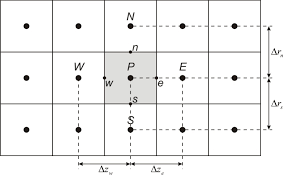
\includegraphics[width=60mm]{Imagens/malha.png}
	\caption{Exemplo de uma malha não adaptativa}
\end{figure}
  	 
  	 
\chapter{Modelo Matemático Diferencial}

\noindent
	
	Uma fração da modelagem matemática já foi citada na introdução. Neste capítulo analisa-se mais detalhadamente essa parte do estudo.
	
\section{Equação da Energia}

\noindent
	
	Como a dedução das equações base não é o foco deste trabalho, a simples citação das relações pode acontecer sem implicar algum dano ao texto.
	
	A relação integral para a equação de energia adequada para um volume de controle fixo é dada na Eq.(\ref{energia})
	
\begin{align}
\label{energia}
Q - We - Wv = \dfrac{\partial}{\partial t}\int\limits_{VC} e \rho dV + \int\limits_{SC}\left(e+\dfrac{p}{\rho}\right) \rho (V n) dA
\end{align}	
	
	Após uma série de considerações e simplificações, é possível reescrever a relação como indicado pela Eq.(\ref{energiadif}).
	
\begin{align}
\label{energiadif}
\rho \dfrac{\partial u}{\partial t} + p (\nabla V) = \nabla (k \nabla T)+ \phi
\end{align}

	Tal equação é válida para um fluido newtoniano sob condições bastante gerais de escoamento não permanente, compressível, viscoso e com codução de calor, desprezando a transferência de calor por radiação e fontes internas de calor. Na Eq.(\ref{energiadif}), o termo $\phi$ equivale à uma abreviação para a função de dissipação viscosa.
	Considerando apenas o processo de difusão, obtém-se a relação dada pela Eq.(\ref{Difusaoone}).

\begin{align}
 \label{Difusao}
 f(x,y,z,t) = \dfrac{\partial \phi}{\partial t} - \alpha \nabla^2 \phi
\end{align}	

\newpage

	Os casos unidimensional e bidimensional são explicitados na introdução, pelas Eq. (\ref{Difuni}) e Eq.(\ref{Difbi}).
	
	Considerando apenas o processo de advecção (com velocidade não nula), obtém-se a relação dada pela Eq.(\ref{Adveccao}).
	
\begin{align}
\label{Adveccao}
f(x,y,z,t) = \dfrac{\partial \phi}{\partial t} + c \nabla \phi
\end{align}

\section{Solução Analítica}

\noindent

	A solução analítica é encontrada através da solução das EDPs indicadas pelas Eq.(\ref{Difusao}) e Eq.(\ref{Adveccao}) quando limitadas à uma ou duas dimensões. Assim, tem-se que a solução analítica para o caso da difusão unidimensional é dado pela Eq.(\ref{soldifun}). As soluções para o caso da advecção unidimensional e bidimensional são dadas pelas Eq.(\ref{soladvuni}) e Eq.(\ref{soladvbi}).
	
\begin{align}
\label{soldifun}
Ue = sen(\theta x) e^{(-\alpha \theta^2 t)}
\end{align}

\begin{align}
\label{soladvuni}
Ue = sen(x - c \ t)
\end{align}

\begin{align}
\label{soladvbi}
Ue = sen(x - cx \ t)sen(y - cy \ t)
\end{align}

	Para a solução analítica da difusão unidimensional fez-se um estudo de otimização de CFL, que possibilitou a redução do erro de segunda ordem para um de quarta ordem. Tal assunto será abordado mais adiante. Para as rotinas regulares da difusão, no entanto, fez-se uso de uma relação que não é solução, sendo assim associada à um termo fonte. A mesma é dada pela Eq.(\ref{difused}) para o caso unidimensional e pela Eq.(\ref{difused2}) para o caso bidimensional.
	
\begin{align}
\label{difused}
Ue = sen(x)[1- e^{(-\theta t)}]
\end{align}

\begin{align}
\label{difused2}
Ue = sen(x) \ sen(y)\ [1- e^{(-\theta t)}] 
\end{align}

\newpage

\section{Condição de Contorno}
\noindent

	Para a difusão e advecção, enquanto eventos separados ou simultâneos, para os casos unidimensional e bidimensional, foi utilizada a condição de contorno de Dirichlet (de primeiro tipo). Assim, a condição de contorno é uma constante conhecida. Para os casos das funções dadas pelas Eq.(\ref{soldifun}),Eq.(\ref{soladvuni}), Eq.(\ref{soladvbi}) e Eq.(\ref{difused}), a condição de contorno obedece à uma senóide, para um domínio fechado de 0 até 2$\pi$, sendo assim de valor nulo.
	Logo, para o caso unidimensional, têm-se as seguintes condições.
	
\begin{align}
\label{eqone}
\phi(0,t) = 0 
\end{align}

\begin{align}
\label{eqtwo}
\phi(2\pi,t) = 0 
\end{align}

	E para o caso bidimensional, têm-se as seguintes relações.
	
\begin{align}
\label{eqthree}
\phi(0,y,t) = 0 
\end{align}

\begin{align}
\label{eqfour}
\phi(2\pi,y,t) = 0
\end{align}

\begin{align}
\label{eqfive}
\phi(x,0,t) = 0
\end{align}

\begin{align}
\label{eqsix}
\phi(x,2\pi,t) = 0
\end{align}
	
\section{Condição Inicial}
\noindent

	Como explicitado anteriormente, o transporte a ser reproduzido é consequente de uma senóide corrigida temporalmente por uma diferença de resposta exponencial com índice negativo. Tal fato se traduz em uma condição inicial de valor nulo, obtida ao substituir o tempo inicial de avaliação nas relações (\ref{difused}) e (\ref{difused2}).
	
	Assim, modela-se um caso em que as relações devem seguir as condições dadas abaixo.

\begin{align}
\label{eqth}
\phi = 0 , \ \forall \ x \ \text{e} \ y 
\end{align}


  	 
  	 \chapter{Modelo Matemático Numérico}


Para discretizar uma equação diferencial, um domínio euleriano foi formulado. Para a velocidade, um método de Runge-kutta de quarta ordem foi aplicado, enquanto a temperatura foi organizada em um esquema de diferenças centradas que tinha que ser resolvido implicitamente. O modelo dinâmico é resolvido primeiro, e seu resultado numérico é utilizado na solução do perfil térmico. O centro da célula estava de tal maneira que a parede era colocada no centro da célula e um ponto entre as células era colocado no centro do canal. A convergência dos resultados numéricos é mostrada na figura \ref{sistema}.

\begin{figure}[!h]
	\centering
	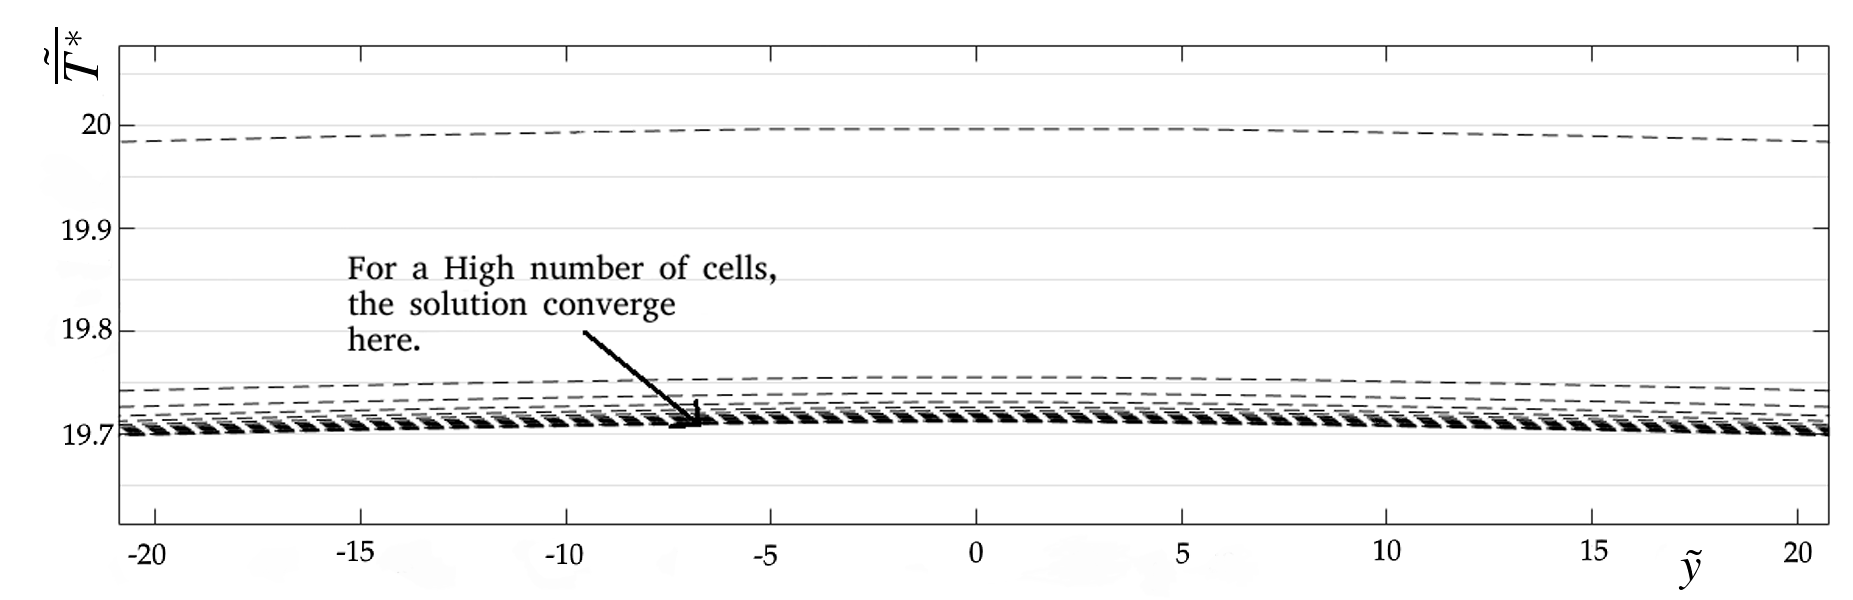
\includegraphics[angle=0, trim={10mm 00mm 0mm 0mm}, clip , scale=0.32]{fotos_formatacao_final/convergnciaprimeira}
	\caption{Convergência do modelo para 400 células.}
	\label{sistema}
\end{figure}
  	 
  	 \chapter{Resultados}

A partir dos resultados iniciais, desenvolveram-se mais e mais modificações para melhorá-los.

\section{Resultados preliminares}
Inicialmente, o número de Prandtl turbulento, $Pr_t = 0.71$, foi usado como o da literatura. Os resultados obtidos são mostrados na figura \ref{figuraresultados1} e comparados com DNS de (Kawamura, 2007) e (kasagi et al., 1992).\\
\begin{figure*}[h!] 
	\centering
	%		\begin{subfigure}[t]{0.49\textwidth}
	%		\centering
	%		\includegraphics[angle=0, scale=0.32]{fotos_formatacao_final/Temperature_150_0025_classico}
	%		\caption{Temperature configuration for $Re_\tau = 150$, $Pr = 0.025$, $L2 = 0.13$ }
	%		\end{subfigure}%
	\begin{subfigure}[t]{0.49\textwidth}
		\centering
		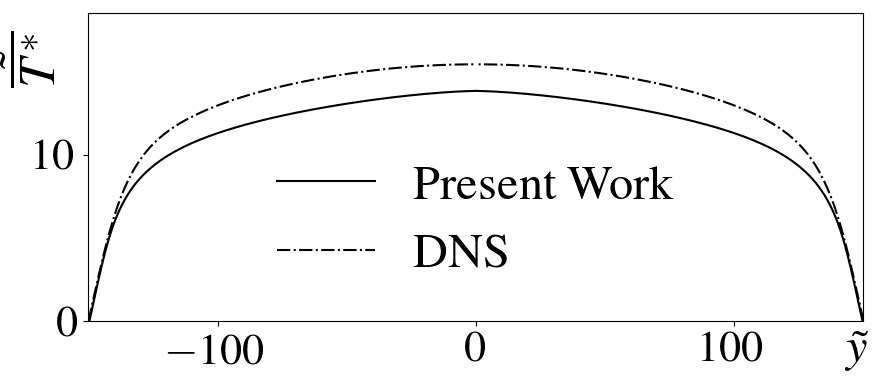
\includegraphics[angle=0, scale=0.24]{fotos_formatacao_final/Temperature_150_071_classico}
		\caption{Distribuição de temperatura para $Re_\tau = 150$, $L2 = 1.42$}
	\end{subfigure}
	%		\begin{subfigure}[t]{0.49\textwidth}
	%		\centering
	%		\includegraphics[angle=0, scale=0.32]{fotos_formatacao_final/Temperature_395_0025_classico}
	%		\caption{Temperature configuration for $Re_\tau = 395$, $Pr = 0.025$, $L2 = 0.52$}
	%		\end{subfigure}%
	\begin{subfigure}[t]{0.49\textwidth}
		\centering
		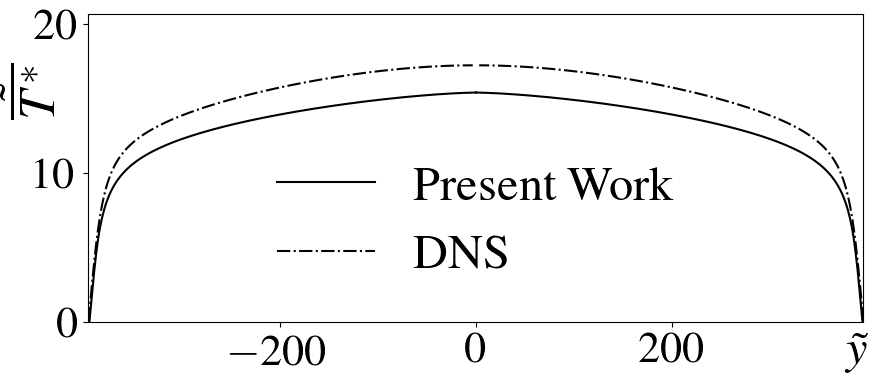
\includegraphics[angle=0, scale=0.24]{fotos_formatacao_final/Temperature_395_071_classico}
		\caption{Distribuição de temperatura para $Re_\tau = 395$, $L2 = 1.55$}
	\end{subfigure}
	%		\centering
	%		\begin{subfigure}[t]{0.49\textwidth}
	%		\centering
	%		\includegraphics[angle=0, scale=0.32]{fotos_formatacao_final/Temperature_395_1_classico}
	%		\caption{Temperature configuration for $Re_\tau = 395$, $Pr = 1.0$, $L2 = 1.89$}
	%		\end{subfigure}%
	%		\begin{subfigure}[t]{0.49\textwidth}
	%		\centering
	%		\includegraphics[angle=0, scale=0.32]{fotos_formatacao_final/Temperature_395_2_classico}
	%		\caption{Temperature configuration for $Re_\tau = 395$, $Pr = 2.0$, $L2 = 2.60$}
	%		\end{subfigure}\\
	%		\begin{subfigure}[t]{0.49\textwidth}
	%		\centering
	%		\includegraphics[angle=0, scale=0.32]{fotos_formatacao_final/Temperature_395_5_classico}
	%		\caption{Temperature configuration for $Re_\tau = 395$, $Pr = 5.0$, $L2 = 3.75$}
	%		\end{subfigure}%
	%		\begin{subfigure}[t]{0.49\textwidth}
	%		\centering
	%		\includegraphics[angle=0, scale=0.32]{fotos_formatacao_final/Temperature_395_7_classico}
	%		\caption{Temperature configuration for $Re_\tau = 395$, $Pr = 7.0$, $L2 = 4.24$}
	%		\end{subfigure}\\
	%	    \centering
	%		\begin{subfigure}[t]{0.49\textwidth}
	%		\centering
	%		\includegraphics[angle=0, scale=0.32]{fotos_formatacao_final/Temperature_395_10_classico}
	%		\caption{Temperature configuration for $Re_\tau = 395$, $Pr = 10.0$, $L2 = 4.55$}
	%		\end{subfigure}%
	%		\begin{subfigure}[t]{0.49\textwidth}
	%		\centering
	%		\includegraphics[angle=0, scale=0.32]{fotos_formatacao_final/Temperature_640_0025_classico}
	%		\caption{Temperature configuration for $Re_\tau = 640$, $Pr = 0.025$, $L2 = 0.84$}
	%		\end{subfigure}\\
	\begin{subfigure}[t]{0.49\textwidth}
		\centering
		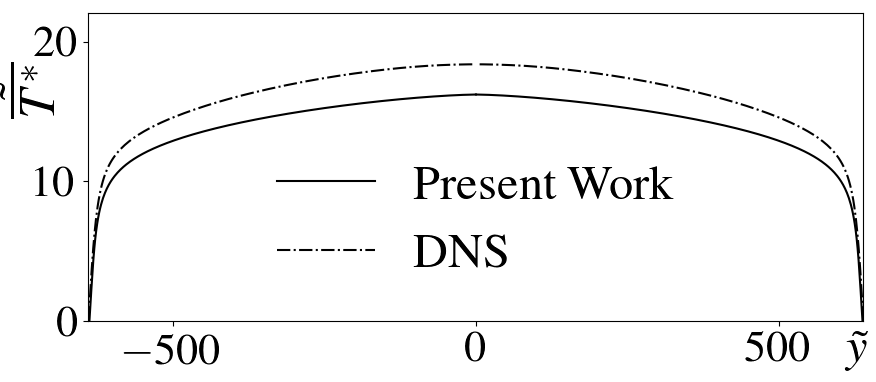
\includegraphics[angle=0, scale=0.24]{fotos_formatacao_final/Temperature_640_071_classico}
		\caption{Distribuição de temperatura para $Re_\tau = 640$, $L2 = 1.79$}
	\end{subfigure}%
	\begin{subfigure}[t]{0.49\textwidth}
		\centering
		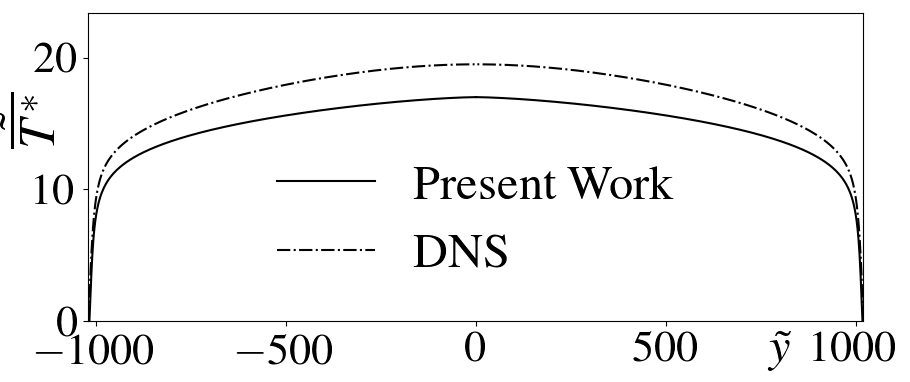
\includegraphics[angle=0, scale=0.24]{fotos_formatacao_final/Temperature_1000_071_classico}
		\caption{Distribuição de temperatura para $Re_\tau = 1020$, $L2 = 2.04$}
	\end{subfigure}%
	\caption{Distribuição de temperatura para $Pr_t = 0.71$, $A = 26$ e $Pr = 0.71$} 
	\label{figuraresultados1}
\end{figure*}	

Os primeiros resultados não foram satisfatórios. Então, notou-se que o número de Prandtl turbulento teve grande influência no resultado, então o número de Prandtl turbulento do DNS (figura \ref{figure5}) foi utilizado como parâmetro no programa, obtendo-se uma norma L2 de $ 0.19 $ para $ Re_t = 640 $. Assim, se observou que o problema se encontrava com a parametrização do número de Prandtl turbulento. Assim, este virou o foco da pesquisa.

\begin{figure*}[h!]
	\centering
	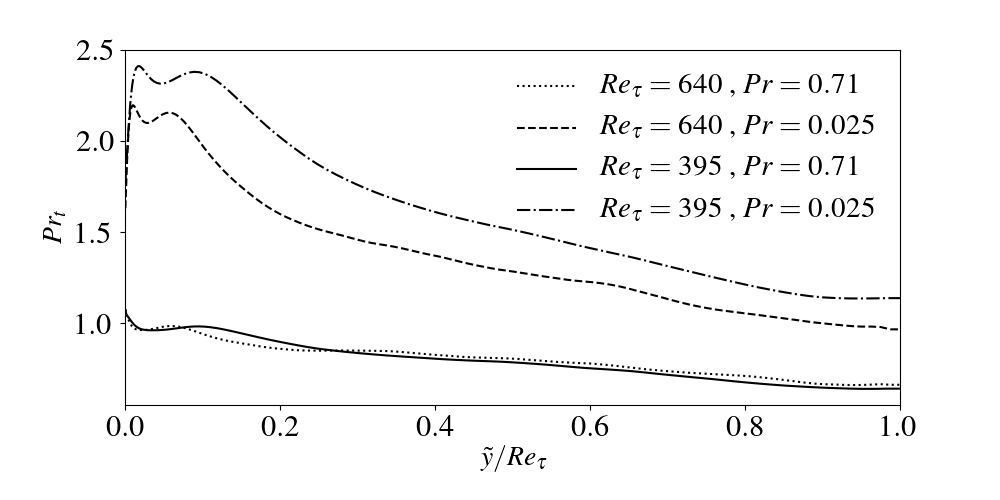
\includegraphics[angle=0, scale=0.4]{fotos_formatacao_final/DNS_PRt}
	\caption{Prandtl do DNS com o número de Prandtl turbulento de acordo com a coordenada $ y $ do canal.}
	\label{figure5}
\end{figure*}

Assim, iniciou-se o esforço para propor uma parametrização ajustada para o número de Prandtl turbulento.
Neste sentido tentou-se ajustar um valor para o qual o erro foi mínimo comparado com o DNS. Neste sentido, a metodologia do algoritmo de evolução diferencial foi aplicada.



\section{A meta-modelagem, com o algoritmo genético: Evolução Diferencial (DE)}
Utilizou-se um algoritmo que buscou um erro mínimo para a função dada, considerando o número de Prandtl turbulento como variável editável e o menor erro como padrão de interesse.
Foi obtido um número de Prandtl turbulento ideal de $ 0.9$ , para o número de Reynolds turbulento de $ 1020$.
\begin{figure}[!h]
	\centering
	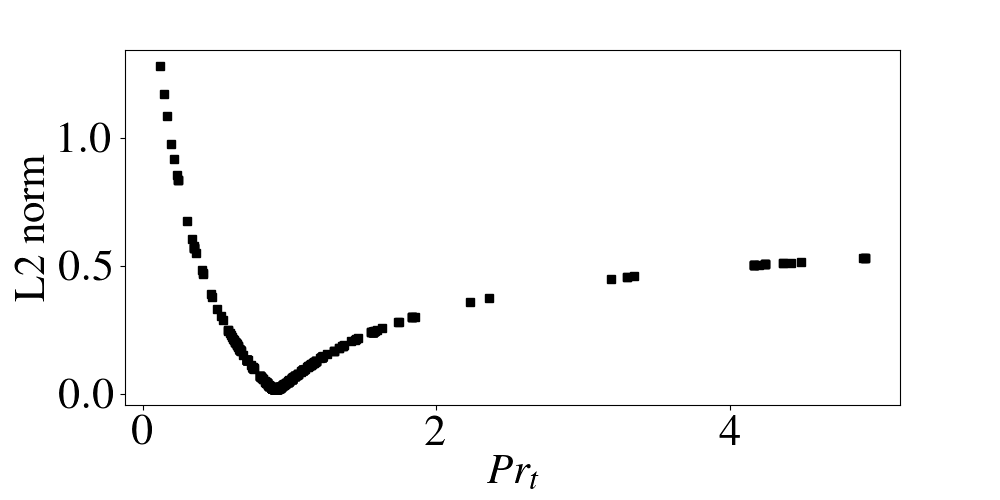
\includegraphics[angle=0, scale=0.31]{fotos_formatacao_final/Genetic_amostra}
	\caption{Iterações do algoritmo genético, com simulações para $Re_\tau = 1020$. Convergência em $Pr_t = 0.9 $.}
\end{figure}

O número de Prandtl turbulento obtido, $Pr_t = 0.9$, foi utilizado nos outros Reynolds turbulento, resultando em:
\begin{figure*}[!h]
	\centering
	\begin{subfigure}[t]{0.5\textwidth}
		\centering
		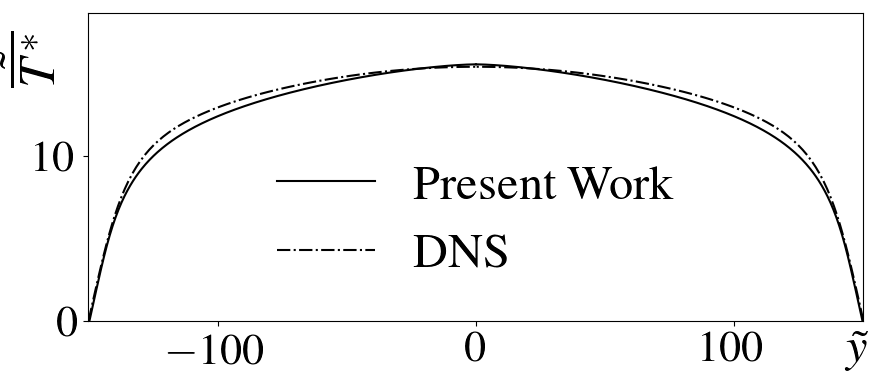
\includegraphics[angle=0, scale=0.24]{fotos_formatacao_final/Temperature_150_071_Prt0905_A26}
		\caption{Distribuição de temperatura para $Re_\tau = 150$, $L2 = 0.34$}
	\end{subfigure}
	\begin{subfigure}[t]{0.45\textwidth}
		\centering
		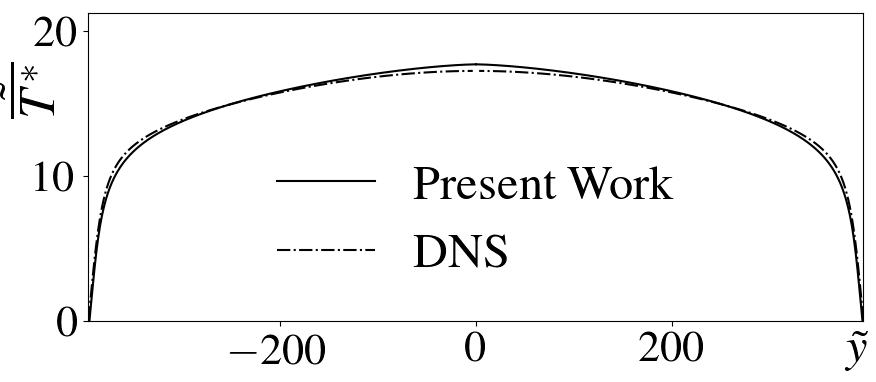
\includegraphics[angle=0, scale=0.24]{fotos_formatacao_final/Temperature_395_071_Prt0905_A26}
		\caption{Distribuição de temperatura para $Re_\tau = 395$, $L2 = 0.23$}
	\end{subfigure}
	\begin{subfigure}[t]{0.5\textwidth}
		\centering
		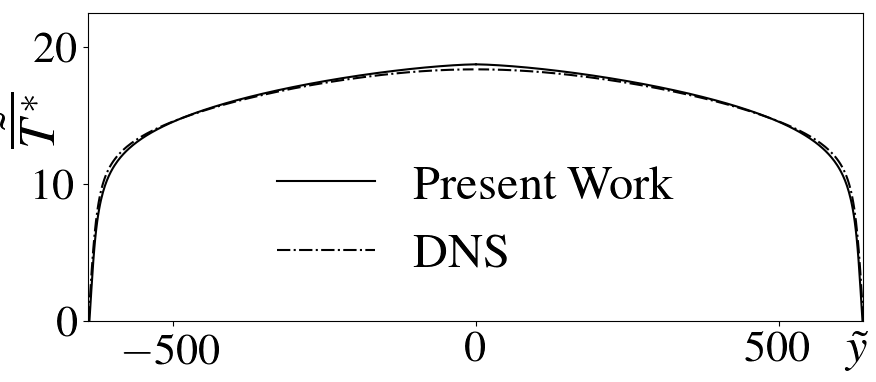
\includegraphics[angle=0, scale=0.24]{fotos_formatacao_final/Temperature_640_071_Prt0905_A26}
		\caption{Distribuição de temperatura para $Re_\tau = 640$, $L2 = 0.19$}
	\end{subfigure}
	\begin{subfigure}[t]{0.45\textwidth}
		\centering
		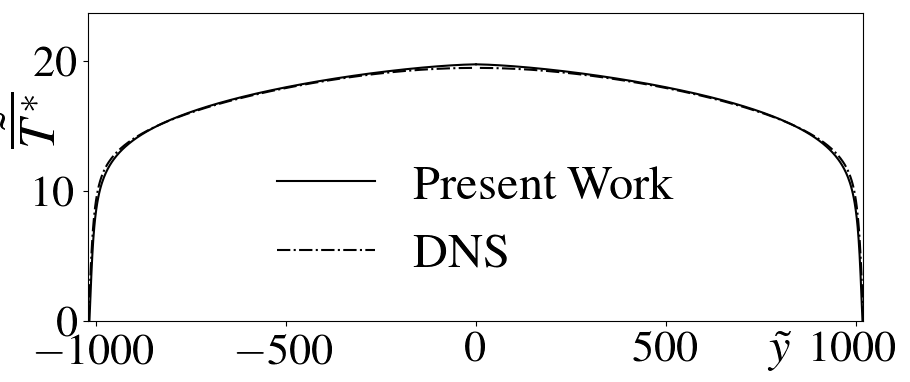
\includegraphics[angle=0, scale=0.24]{fotos_formatacao_final/Temperature_1000_071_Prt0905_A26}
		\caption{Distribuição de temperatura para $Re_\tau = 1020$, $L2 = 0.14$}
	\end{subfigure}	
	\caption{Resultado de simulações térmicas para $Pr_t = 0.9 $, $A = 26$ e $Pr =0.71$ }
\end{figure*}

Mesmo os resultados sendo muito melhores quando comparados ás figuras \ref{figuraresultados1}, o modelo tinha que ser melhorado. O número de Prandtl turbulento variava com o número de Reynolds turbulento, como visto em (fig.\ref{figure5}), assim, um modelo que contemplasse esse fato tinha de ser proposto. 
Para se obter uma curva para o $Pr_t$ em função de $Re_\tau$, o mesmo algoritmo de otimização teve que ser usado para determinar um número de Prandtl turbulento ideal para cada número de Reynolds turbulento disponível na base de dados de DNS. (Kawamura, 2007) e (kasagi et al., 1992).
Os melhores números de Prandtl turbulentos obtidos foram:

\begin{table}[!h]
	\centering
	\caption{Números de Prandtl turbulentos ideais ajustados para cada número de Reynolds turbulento, com $A = 26$}
	\begin{tabular}{ll}
		\hline
		$Re_\tau$ & $Pr_t$\\
		\hline
		150  &   0.94531\\
		395  &   0.89531\\
		640  &   0.89531\\
		1020 &   0.90000\\ 
		\hline
	\end{tabular}
\end{table}



Executando um ajuste de curva polinomial, um modelo ajustado para o número de Prandtl turbulento como uma função do número de Reynolds turbulento foi desenvolvido:
\begin{equation}
\begin{split}
Pr_t = -4.5604 * 10^{-10} Re_\tau^3 + 9.5690 * 10^{-7} Re_\tau^2 - 6.1715 *10 ^{-4} Re_\tau + 1.0178 
\end{split}
\end{equation}
Os resultados das simulações foram muito precisos, ainda mais do que as simulações com os números de Prandtl turbulentos definidos como os valores médios dos dos dados do DNS. (fig.\ref{figure5}). Estes foram:



\begin{figure*}[!h]
	\centering
	\begin{subfigure}[t]{0.5\textwidth}
		\centering
		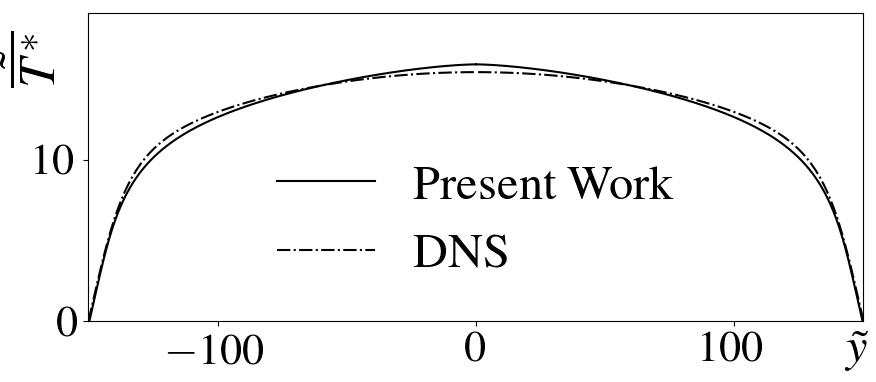
\includegraphics[angle=0, scale=0.24]{fotos_formatacao_final/Temperature_150_071_Prt(Ret)_A26}
		\caption{Distribuição de temperatura para $Re_\tau = 150$, $L2 = 0.26$}
	\end{subfigure}
	\begin{subfigure}[t]{0.45\textwidth}
		\centering
		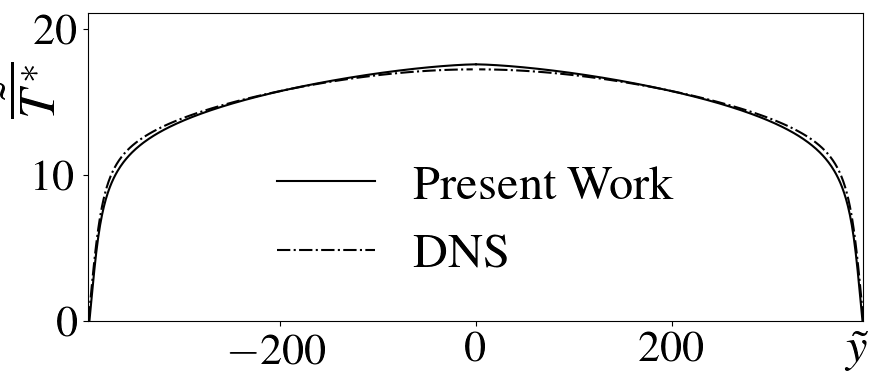
\includegraphics[angle=0, scale=0.24]{fotos_formatacao_final/Temperature_395_071_Prt(Ret)_A26}
		\caption{Distribuição de temperatura para $Re_\tau = 395$, $L2 = 0.22$}
	\end{subfigure}
	\begin{subfigure}[t]{0.5\textwidth}
		\centering
		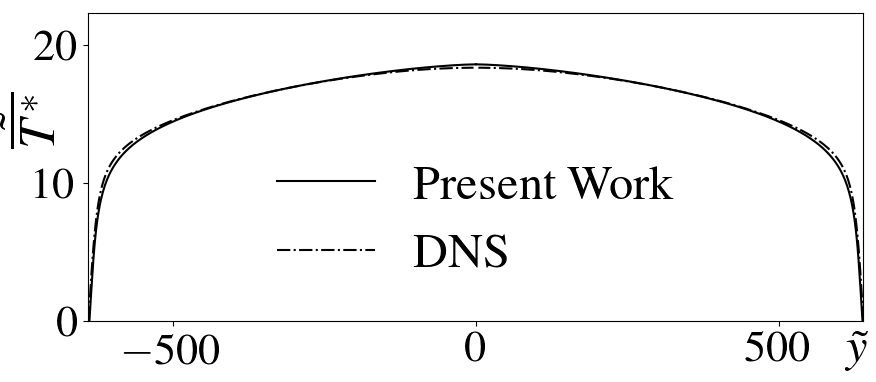
\includegraphics[angle=0, scale=0.24]{fotos_formatacao_final/Temperature_640_071_Prt(Ret)_A26}
		\caption{Distribuição de temperatura para $Re_\tau = 640$, $L2 = 0.17$}
	\end{subfigure}
	\begin{subfigure}[t]{0.45\textwidth}
		\centering
		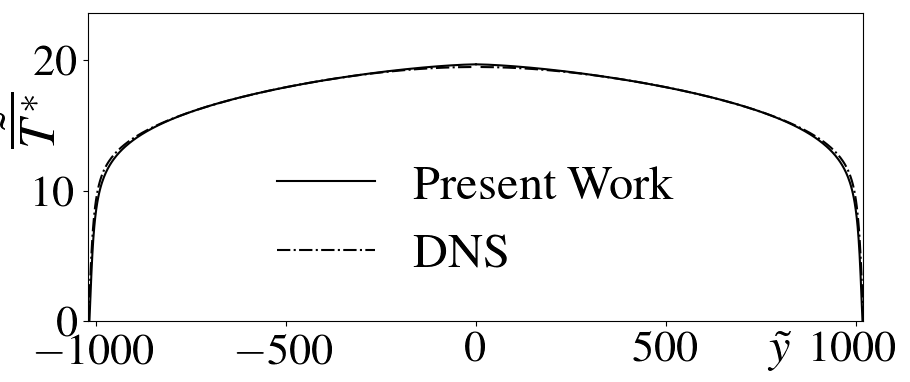
\includegraphics[angle=0, scale=0.24]{fotos_formatacao_final/Temperature_1000_071_Prt(Ret)_A26}
		\caption{Distribuição de temperatura para $Re_\tau = 1020$, $L2 = 0.14$}
	\end{subfigure}	
	\caption{Resultados de simulações térmicas para $Pr_\tau(Re_\tau)$, $A = 26$ e $Pr =0.71$ }
\end{figure*}



\newpage

Outras maneiras de reduzir a imprecisão foram pesquisadas. O perfil de velocidade foi uma possibilidade, uma vez que desempenha um papel importante no erro do método. Simulações foram realizadas desenvolvendo apenas essa propriedade física, e houve erro associado, como pode ser visto adiante:

\begin{figure*}[!h]
	\centering
	\begin{subfigure}[t]{0.5\textwidth}
		\centering
		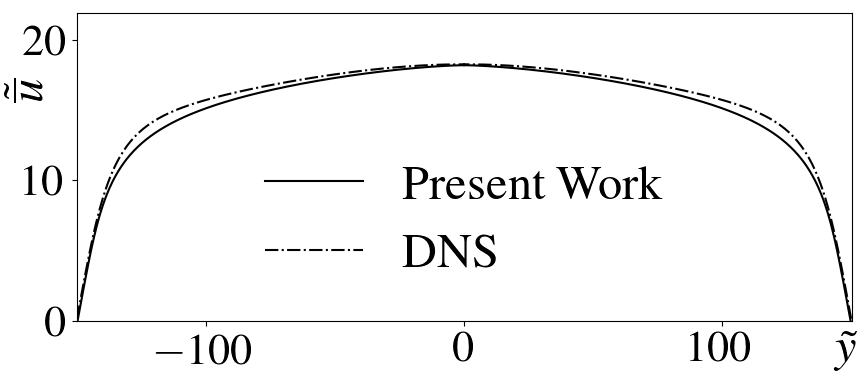
\includegraphics[angle=0, scale=0.24]{fotos_formatacao_final/Temperature_150_Avelocity}
		\caption{Distribuição de velocidade para $Re_\tau = 150$, $L2 = 0.47$}
	\end{subfigure}
	\begin{subfigure}[t]{0.45\textwidth}
		\centering
		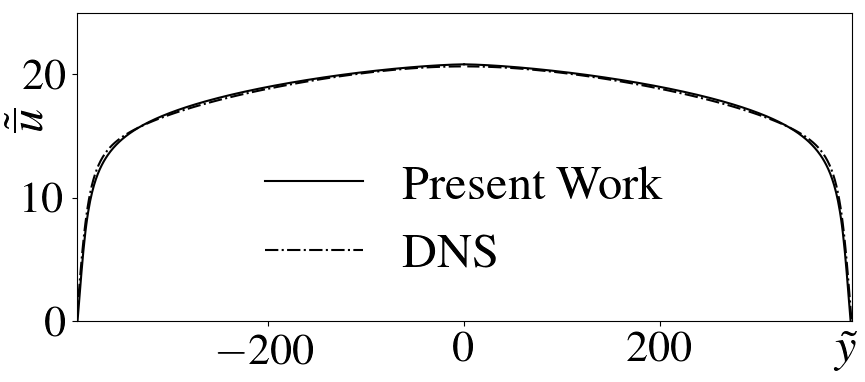
\includegraphics[angle=0, scale=0.24]{fotos_formatacao_final/Temperature_395_Avelocity}
		\caption{Distribuição de velocidade para $Re_\tau = 395$, $L2 = 0.17$}
	\end{subfigure}
	\begin{subfigure}[t]{0.5\textwidth}
		\centering
		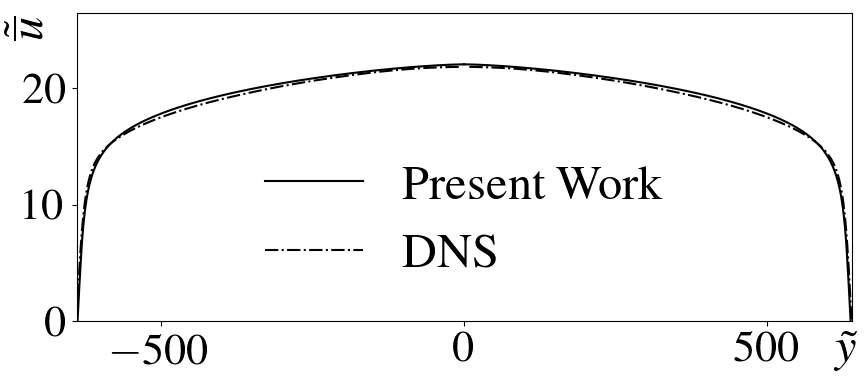
\includegraphics[angle=0, scale=0.24]{fotos_formatacao_final/Temperature_640_Avelocity}
		\caption{Distribuição de velocidade para $Re_\tau = 640$, $L2 = 0.23$}
	\end{subfigure}
	\begin{subfigure}[t]{0.45\textwidth}
		\centering
		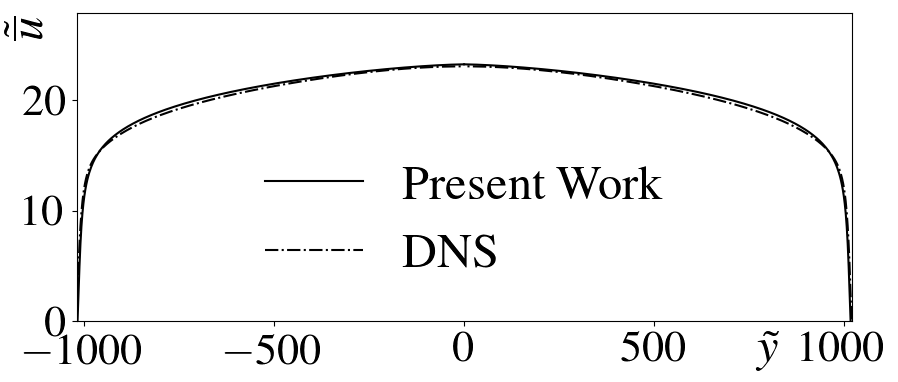
\includegraphics[angle=0, scale=0.24]{fotos_formatacao_final/Temperature_1000_Avelocity}
		\caption{Distribuição de velocidade para $Re_\tau = 1020$, $L2 = 0.23$}
	\end{subfigure}	
	\caption{Resultados de simulações dinâmicas para $A = 26$}
\end{figure*}

Um modelo ajustado foi preparado no presente trabalho para a constante de Cebeci $A$ com o objetivo de reduzir o erro e, por extensão, tornar o método mais preciso. O mesmo algoritmo usado para encontrar os números ideais de Prandtl turbulento foi usado para encontrar uma constante de Cebecis ideal para cada número de Reynolds turbulento. Foi utilizada a velocidade do DNS disponível para calcular a norma L2. A constante de Cebeci "A" foi definida como uma variável editável para o programa, e a norma L2 foi definida como um parâmetro de interesse. Os resultados para as constantes ideais do Cebeci podem ser vistos adiante:


\begin{table}[!h]
	\centering
	\caption{Constantes de Cebeci ideais ajustadas para cada Reynolds turbulento.}
	\begin{tabular}{ll}
		\hline
		$Re_\tau$ & $A$\\
		\hline
		150  &   28.616180\\
		395  &   25.673782\\
		640  &   25.001266\\
		1020 &   25.002136\\ 
		\hline
	\end{tabular}
	\label{tablea}
\end{table}

Dos pontos resultantes do algoritmo de otimização, um modelo de função de Cebeci fora ajustado:
\begin{equation}
A = \frac{Re_\tau ^{0.04510621 * \ln(Re_\tau)} *e ^ {5.27528132} }{Re_\tau ^{0.60941173}}
\end{equation}

Em seguida, foram feitas simulações com a função otimizada para um erro mínimo em relação à velocidade, como pode ser visto nas simulações, houve uma melhora nos resultados:


\begin{figure*}[!h]
	\centering
	\begin{subfigure}[t]{0.5\textwidth}
		\centering
		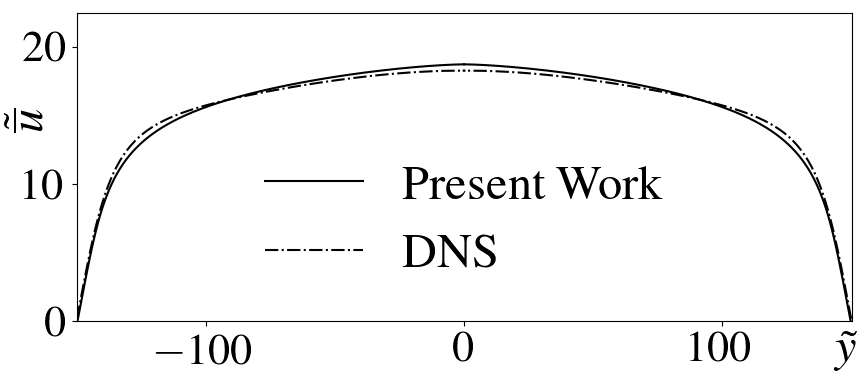
\includegraphics[angle=0, scale=0.24]{fotos_formatacao_final/Temperature_150_Amodeled}
		\caption{Distribuição de velocidade para $Re_\tau = 150$, $L2 = 0.28$}
	\end{subfigure}
	\begin{subfigure}[t]{0.45\textwidth}
		\centering
		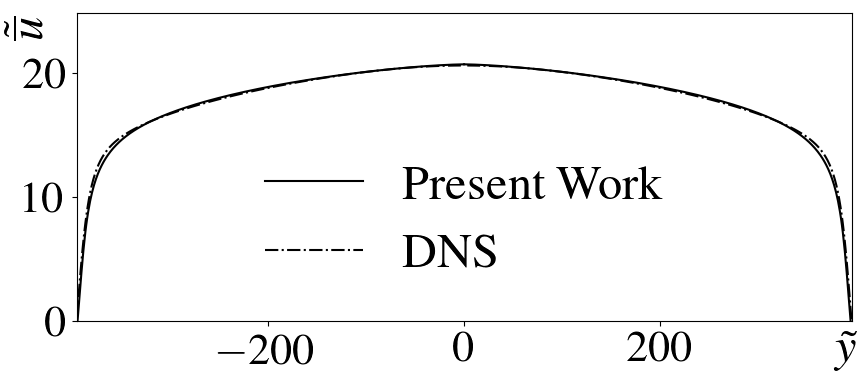
\includegraphics[angle=0, scale=0.24]{fotos_formatacao_final/Temperature_395_Amodeled}
		\caption{Distribuição de velocidade para $Re_\tau = 395$, $L2 = 0.16$}
	\end{subfigure}
	\begin{subfigure}[t]{0.5\textwidth}
		\centering
		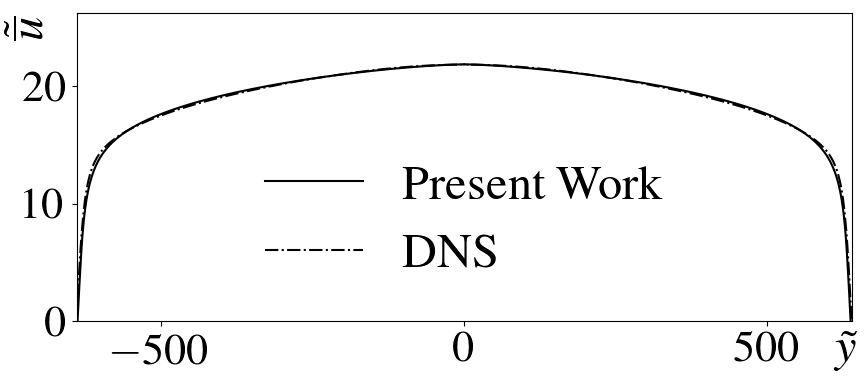
\includegraphics[angle=0, scale=0.24]{fotos_formatacao_final/Temperature_640_Amodeled}
		\caption{Distribuição de velocidade para $Re_\tau = 640$, $L2 = 0.14$}
	\end{subfigure}
	\begin{subfigure}[t]{0.45\textwidth}
		\centering
		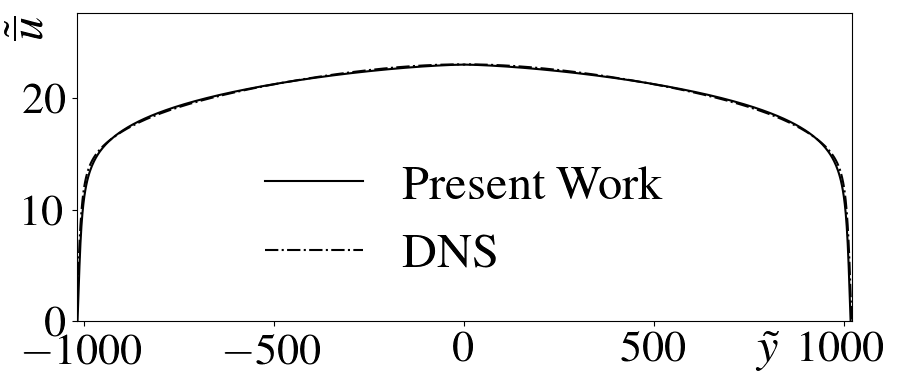
\includegraphics[angle=0, scale=0.24]{fotos_formatacao_final/Temperature_1000_Amodeled}
		\caption{Distribuição de velocidade para $Re_\tau = 1020$, $L2 = 0.13$}
	\end{subfigure}	
	\caption{Resultados para a velocidade com o valor de Cebeci modelado.}
\end{figure*}

Com a função do Cebeci ajustada, um novo grupo de otimizações foi feito, com a mesma metodologia de evolução diferencial, levando em consideração essa nova formulação para a constante do Cebeci. Esse estudo resultou em um novo conjunto de números ótimos de Prandtl turbulentos para cada número de Reynolds de amostra de DNS, como segue:


\begin{table}[!h]
	\centering
	\caption{Números de Prandtl turbulentos ideais ajustados para cada número de Reynolds turbulento, com A modelado.}
	\begin{tabular}{ll}
		\hline
		$Re_\tau$ & $Pr_t$\\
		\hline
		150  &   0.88594\\
		395  &   0.90156\\
		640  &   0.91094\\
		1020 &   0.91406\\ 
		\hline
	\end{tabular}
\end{table}

Um novo modelo pôde ser proposto para o número de Prandtl Turbulento:
\vspace{-2mm}
\begin{equation}
\begin{split}
Pr_t = 4.5290 * 10^{-12} Re_\tau^3 - 5.73952 * 10^{-8} Re_\tau^2 + 9.397 * 10^{-5} Re_\tau + 0.873117480.
\end{split}
\end{equation}


Com essa parametrização, foi feito um novo conjunto de simulações, com os seguintes resultados:

\begin{figure*}[!h]
	\centering
	\begin{subfigure}[t]{0.5\textwidth}
		\centering
		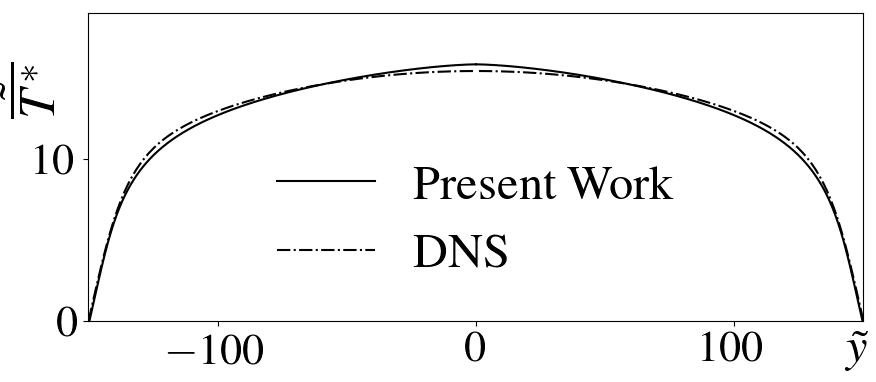
\includegraphics[angle=0, scale=0.24]{fotos_formatacao_final/Temperature_150_071_Prt(Ret)_Avelocity}
		\caption{Distribuição de temperatura para $Re_\tau = 150$, $L2 = 0.212$}
	\end{subfigure}
	\begin{subfigure}[t]{0.45\textwidth}
		\centering
		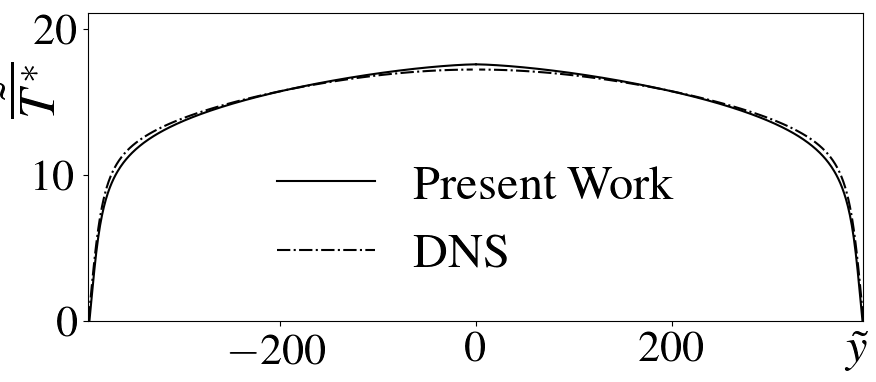
\includegraphics[angle=0, scale=0.24]{fotos_formatacao_final/Temperature_395_071_Prt(Ret)_Avelocity}
		\caption{Distribuição de temperatura para $Re_\tau = 395$, $L2 = 0.233$}
	\end{subfigure}
	\begin{subfigure}[t]{0.5\textwidth}
		\centering
		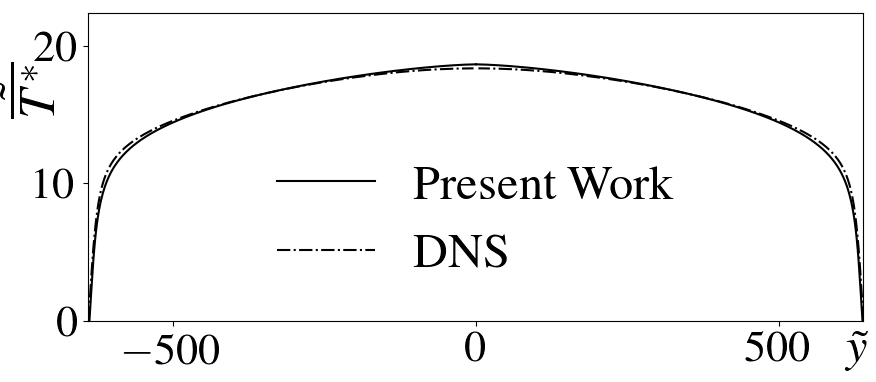
\includegraphics[angle=0, scale=0.24]{fotos_formatacao_final/Temperature_640_071_Prt(Ret)_Avelocity}
		\caption{Distribuição de temperatura para $Re_\tau = 640$, $L2 = 0.205$}
	\end{subfigure}
	\begin{subfigure}[t]{0.45\textwidth}
		\centering
		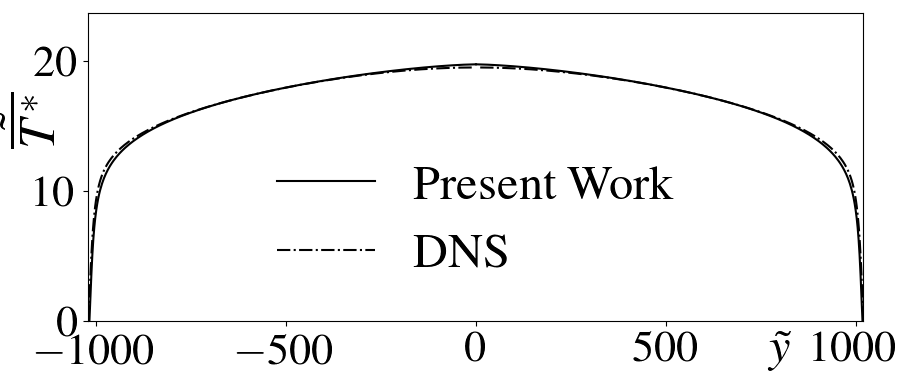
\includegraphics[angle=0, scale=0.24]{fotos_formatacao_final/Temperature_1000_071_Prt(Ret)_Avelocity}
		\caption{Distribuição de temperatura para $Re_\tau = 1020$, $L2 = 0.175$}
	\end{subfigure}	
	\caption{Resultado para simulações térmicas para $Pr_\tau(Re\tau)$, $A(Re_\tau)$ and $Pr =0.71$ }
\end{figure*}

Os valores do Cebeci que resultaram em um pequeno erro para o algoritmo da velocidade não tiveram o mesmo efeito nos resultados de temperatura. O Cebeci foi modelado para o erro de velocidade mínima, não sendo o melhor para a solução térmica. Algebricamente, a constante de Cebeci aparece duas vezes como se vê nas equações \ref{equationultima} e \ref{finalequationvelocity}. Então, é possível propor dois modelos de constantes de Cebeci. Um para a simulação dinâmica e outro para a simulação de temperatura.    


Outro método de ajuste na evolução diferencial é o ajuste multi objetivo. Tal abordagem foi usada para considerar mais de uma variável simultaneamente para otimização. Este método foi usado para ajustar a constante de Cebeci térmica e o número de Prandtl Turbulento para o menor erro (norma L2) no campo de temperatura resultante para cada amostra de DNS. A função dinâmica de Cebeci foi considerada a anteriormente desenvolvida. Novos valores ideais foram encontrados para o número de Prandtl turbulento e a constante térmica de Cebeci:

\begin{table}[!h]
	\centering
	\caption{Números de Prandtl turbulentos ideais e constantes de Cebeci ajustadas para cada número turbulento de Reynolds, com a abordagem multi objetiva. O Cebeci dinâmico continuou o mesmo da tabela \ref{tablea}. }
	\begin{tabular}{llll}
		\hline
		$Re_\tau$ & $Pr_t$ & $A_d$ & $A_v$\\
		\hline
		150  &   0.72530 & 37.25510 & 28.616180\\
		395  &   0.76821 & 34.24176 & 25.673782\\
		640  &   0.81896 & 31.27627 & 25.001266\\
		1020 &   0.86179 & 28.73726 & 25.002136\\ 
		\hline
	\end{tabular}
\end{table}
Com tais dados numéricos, foram propostos novos modelos para o número de Prandtl Turbulento e a constante térmica de Cebeci:

\begin{equation}
A_t = \frac{Re_\tau ^{0.0395059904287 \ln(Re_\tau)^2 - 0.758759596012 \ln(Re_\tau) +  4.66369525666  } }{e ^{5.67034263}}
\end{equation}

\begin{equation}
\begin{split}
Pr_t = -2.4891 * 10^{-10} Re_\tau^3 +  3.60362 * 10^{-7} Re_\tau^2 + 3.7921 *10 ^{-5} Re_\tau + 0.71234 
\end{split}
\end{equation}
Novas simulações foram desenvolvidas com essa parametrização:

\begin{figure*}[!h]
	\centering
	\begin{subfigure}[t]{0.5\textwidth}
		\centering
		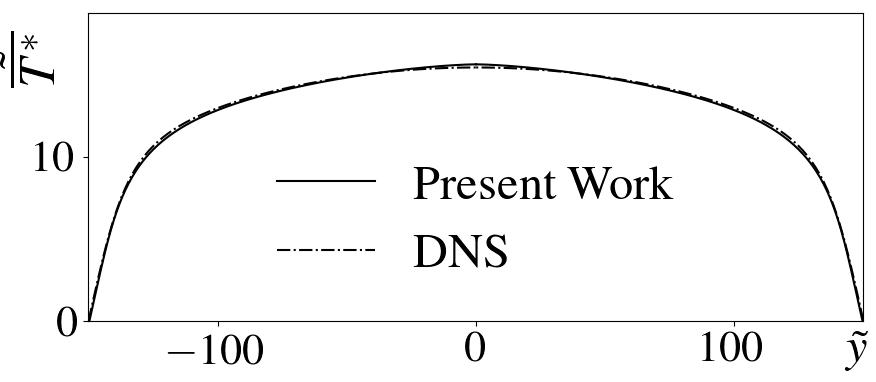
\includegraphics[angle=0, scale=0.24]{fotos_formatacao_final/Temperature_150_071_Genetic2temperature}
		\caption{Distribuição de temperatura para $Re_\tau = 150$, $L2 = 0.091$}
	\end{subfigure}
	\begin{subfigure}[t]{0.45\textwidth}
		\centering
		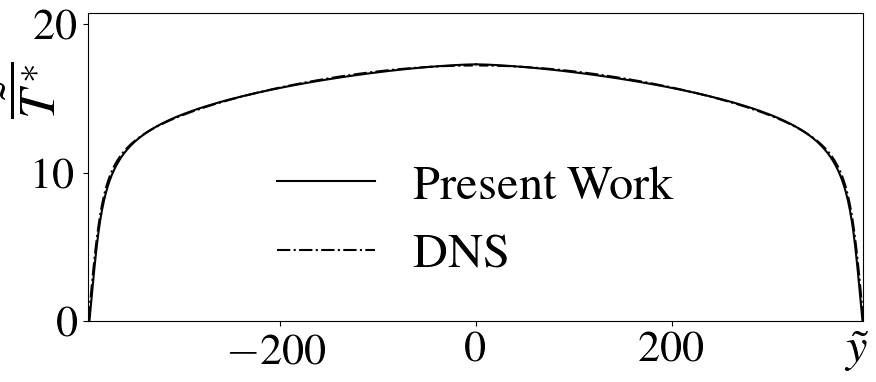
\includegraphics[angle=0, scale=0.24]{fotos_formatacao_final/Temperature_395_071_Genetic2temperature}
		\caption{Distribuição de temperatura para $Re_\tau = 395$, $L2 = 0.049$}
	\end{subfigure}
	\begin{subfigure}[t]{0.5\textwidth}
		\centering
		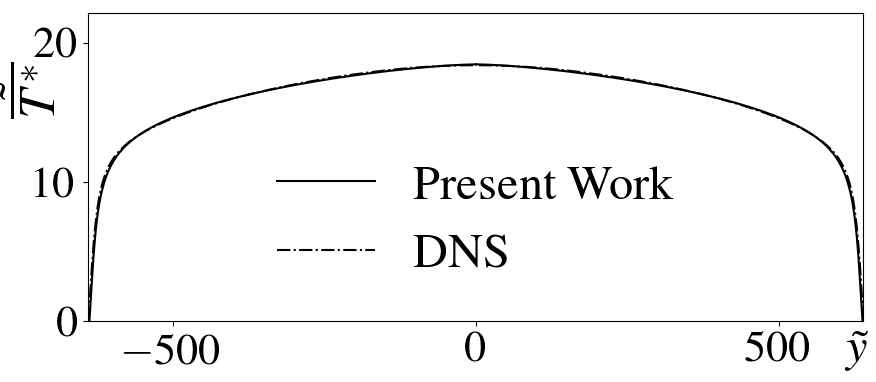
\includegraphics[angle=0, scale=0.24]{fotos_formatacao_final/Temperature_640_071_Genetic2temperature}
		\caption{Distribuição de temperatura para $Re_\tau = 640$, $L2 = 0.061$}
	\end{subfigure}
	\begin{subfigure}[t]{0.45\textwidth}
		\centering
		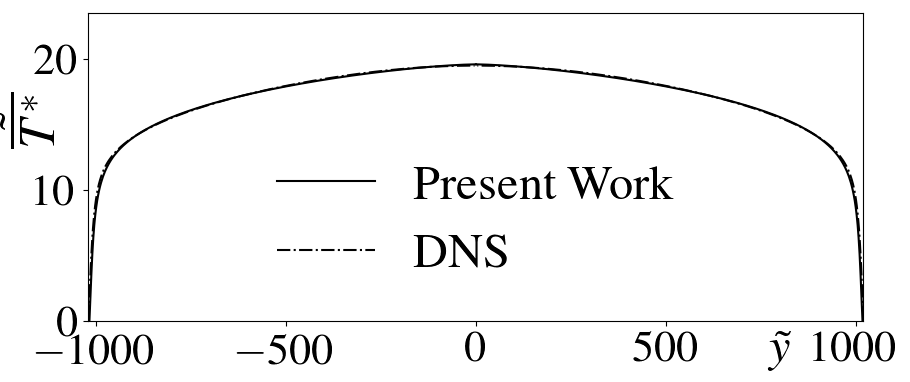
\includegraphics[angle=0, scale=0.24]{fotos_formatacao_final/Temperature_1000_071_Genetic2temperature}
		\caption{Distribuição de temperatura para $Re_\tau = 1020$, $L2 = 0.076$}
	\end{subfigure}	
	\caption{Resultados de simulações térmicas para $Pr_\tau(Re_\tau)$, $A_d(Re_\tau)$, $A_t(Re_\tau) $ e $Pr =0.71$, com ajuste multi objetivo.}
	\vspace{-5mm}
\end{figure*}



\chapter{Discussão}


\section{Resultados}

Com esses métodos, foram estudadas as vantagens e desvantagens de cada um. Uma comparação entre seus erros pode ser vista adiante:\\

\begin{figure}[!h]
	\centering
	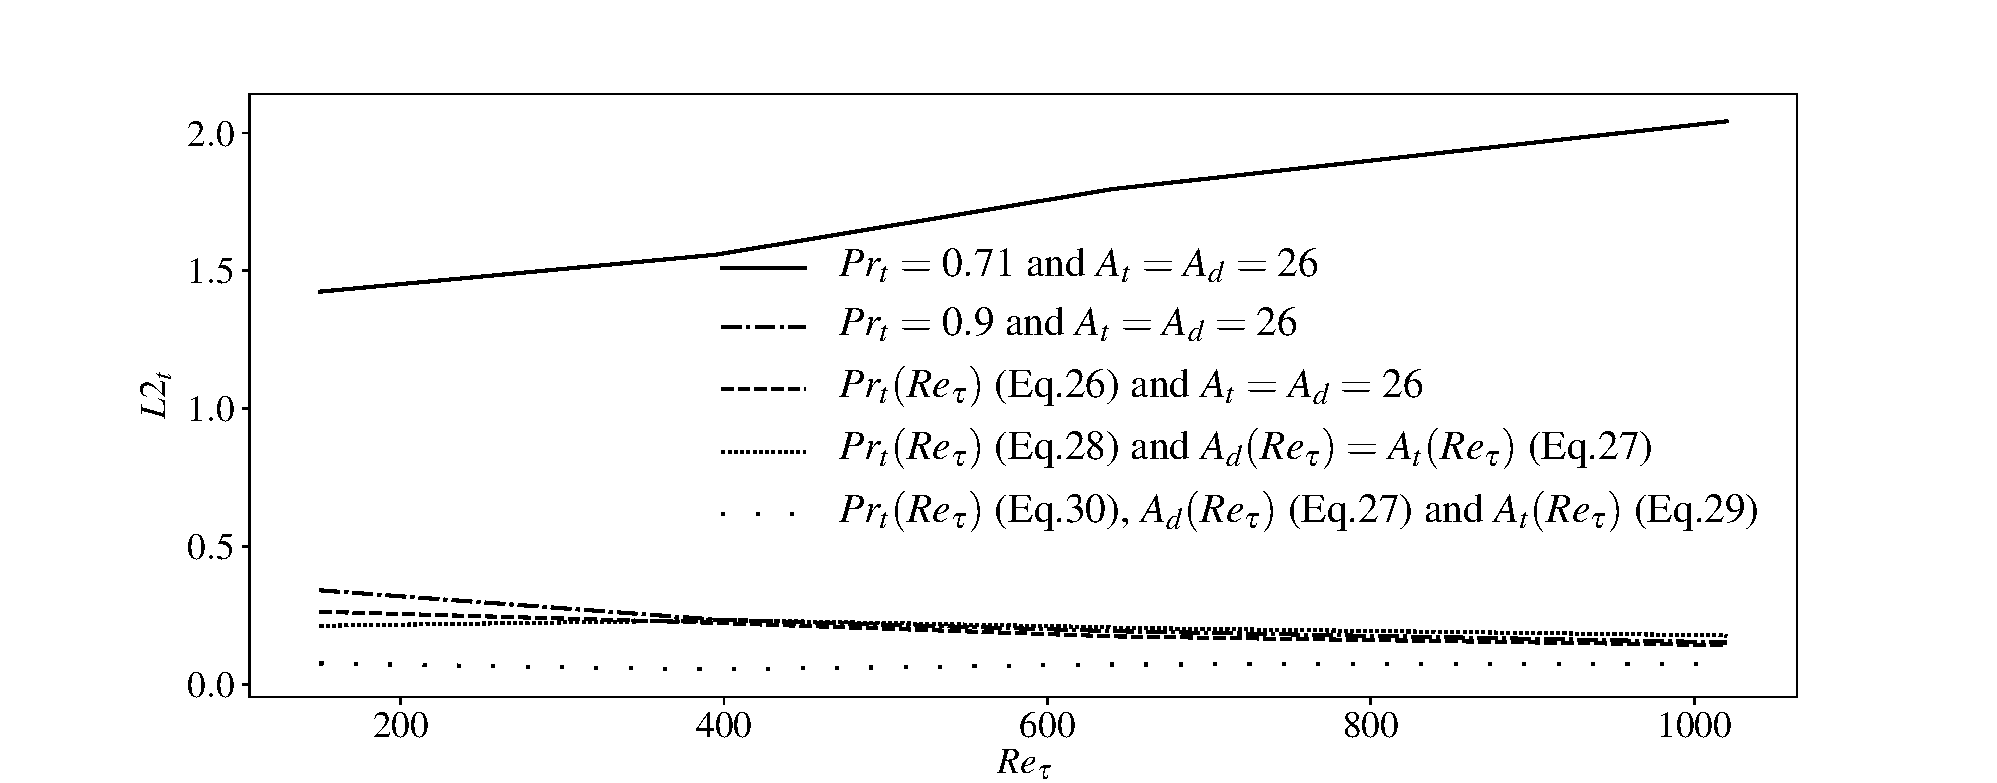
\includegraphics[angle=0, trim = {0mm 0mm 0mm 10mm}, scale=0.5]{fotos_formatacao_final/gerais}
	\caption{Comparison between all parameterizations for $Re_\tau$ and $Pr_t$.}
\end{figure}

Todos os modelos desenvolvidos no presente trabalho apresentaram melhores resultados que a parametrização clássica de $ Pr_t = 0.71 $ e $ A = 26 $ no escoamento turbulento de Poiseuille. A correção na constante do Cebeci, apesar de representar um erro menor na velocidade, não resultou em erros menores no perfil de temperatura para todo o domínio. O modelo que obteve os melhores resultados foi o desenvolvido com o algoritmo de evolução diferencial multi-objetivo em que foram considerados dois valores de Cebeci para cada domínio (térmico e dinâmico).

\section{Conclusões}

No presente trabalho foi desenvolvido com sucesso uma metodologia semi-analítica para calcular o perfil de temperatura em um canal com o modelo de comprimento de mistura Prandtl, um modelo clássico de fechamento no estudo da turbulência. As validações com o DNS foram satisfatórias. É importante notar que tais valores do número de Prandtl turbulento e constante de Cebeci foram aplicados para este caso particular, pois as parametrizações foram ajustes computacionais particulares e são simplificações das abstrações físicas que cada problema representa. Mas eles se adaptaram bem a este caso, resultando em precisão e eficiência. O método semi analítico foi bem sucedido no modelo do problema, pois bons resultados foram obtidos quando utilizados os números de Prandtl turbulento do DNS. Quanto aos modelos propostos, é uma ideia o aplicar então em outros problemas, com outras geometrias, como forma de testar sua universalidade.
  	 
  	 \newpage
  	 
  	 \begin{large}
\textbf{Referências Bibliográficas}
\end{large} 
\\
\\
Ferziger, J. H. and Peric, M., 2001. Computational Methods for Fluid Dynamics. \\ \\
Fortuna, A. O, 2012. Técnicas Computacionais para Dinâmica dos Fluidos. \\ \\
LeVeque, R. J., 2002. Finite Volume Method for Hyperbolic Problems. \\ \\
LeVeque, R. J., 2007. Finite Difference Method for Ordinary and Partial Differential
Equations. \\ \\
LeVeque, R. J., 1992. Numerical Methods for Conservation Laws. \\ \\
Maliska, C. R. Transferência de Calor e Mecânica dos Fluidos Computacional:
Fundamentos e Coordenadas Generalizadas, 1st Ed. 250 p. LTC, Rio de Janeiro, 1995. \\ \\
Patankar, S. V., 1980. Numerical heat transfer and fluid flow (series in computational
methods in mechanics as thermal sciences). \\ \\
Pivello, M. R., 2012. Um método front-tracking completamente adaptativo para a
simulação de escoamentos tridimensionais bifásicos. Tese de Doutorado, Universidade
Federal de Uberlândia. \\ \\
Roma, A. M., 1996. A Multilevel self-adaptive version of the immersed boundary
method. Ph.D. Thesis, New York University, 1996. \\ \\
Salari, K. and Knupp, P., 2000. Code Verification by the Method of Manufactured
Solutions. Report, Sandia Corporation, California. \\ \\
Villar, M. M., 2007. Análise numérica detalhada de escoamentos multifásicos
bidimensionais. Tese de Doutorado, Universidade Federal de Uberlândia. \\ \\
White, F. M. Fluid Mechanics. 4. ed. New York, NY, USA: McGraw-Hill, 1998.
(McGraw-Hill Series in Mechanical Engineering). \\

%
%\begin{large}
%\textbf{Nota de responsabilidade}
%\end{large} 
%\\
%\\
%	Os autores são responsáveis por todo o material disponibilizado no presente trabalho.
  	 
  \end{document}